\documentclass{article} % For LaTeX2e
\usepackage{iclr2027_conference,times}
% Local XeTeX/tectonic builds have no Times metrics and silently drop bold; Overleaf's pdflatex is unaffected.
\usepackage{ifxetex}\ifxetex\usepackage{fontspec}\setmainfont{Liberation Serif}\fi

\input{math_commands.tex}

\usepackage{hyperref}
\usepackage{url}
\usepackage{booktabs}
\usepackage{graphicx}
\usepackage{amsmath,amssymb,amsthm}
\usepackage{multirow}
\usepackage{xcolor}

% FIRST DRAFT (2026-09-15) for advisor review. Every table body lives in data/tables/*.tex and is
% regenerated by scripts/make_tables.py from ../results/*.json; nothing is typed by hand.
% Two visible draft macros, to be removed before submission:
%   \todo{...}         work not yet done
%   \provisional{...}  a claim whose supporting run is still in the queue (listed in ../PLAN.md)
\newcommand{\todo}[1]{\textcolor{red}{[TODO: #1]}}
\newcommand{\provisional}[1]{\textcolor{blue}{#1}}

\newtheorem{proposition}{Proposition}
\newtheorem{lemma}{Lemma}
\newtheorem{corollary}{Corollary}

% Notation (kept consistent with the certificate's source paper, Sec. 3):
%   pool D of N examples x = (prompt, response); property u(x) in {0,1} (1 = harmful);
%   score g(x); threshold lambda; selection S(lambda) = {x : g(x) >= lambda};
%   calibration sample C of n labeled examples; N_j, m_j, k_j at grid point j;
%   target alpha, confidence delta; realized composition alpha-hat = mean of u over S.
\newcommand{\pool}{\mathcal{D}}
\newcommand{\calset}{\mathcal{C}}
\newcommand{\sel}[1]{S(#1)}
\newcommand{\ahat}{\hat\alpha}
\makeatletter
\newcommand{\tabinput}[1]{\@@input#1 }
\makeatother

\title{Clean Data, Unsafe Model: Certified Safety Curation for LLM Fine-Tuning}

\author{Adam Haroon\thanks{Corresponding author: \texttt{aharoon@iastate.edu}}, \ Cody Fleming \\
Iowa State University\\
Ames, IA, USA\\
\texttt{\{aharoon,flemingc\}@iastate.edu}}

\iclrfinalcopy

\begin{document}

\maketitle
% Header modes, as in the RL paper:
%   PREPRINT (current): \iclrfinalcopy + this \lhead override -> authors shown, header "Preprint. Under review."
%   ICLR SUBMISSION: remove \iclrfinalcopy (anonymous) and this \lhead line (template prints "Under review ...").
%   CAMERA-READY: keep \iclrfinalcopy, remove the \lhead override.
\lhead{Preprint. Under review.}

\begin{abstract}
A fine-tuned model needs safe examples of harmful prompts as much as it needs few harmful examples, and judge-based filters remove exactly those. We bring to fine-tuning data a distribution-free certificate: given any scorer and a few hundred human labels, it returns a cutoff whose kept set is at most an $\alpha$-fraction harmful with probability $1 - \delta$, or refuses. On BeaverTails its guarantee holds and a closed form predicts its label budget. A certified set then exposes what else a filter does. At 0.5B, a judge-selected set certified at most $10$ percent harmful trains a more harmful model than the pool, because the judge scores a response by its prompt and discards the demonstrations. On an aligned 8B model the same judge, asked SAFT's question, keeps a set more harmful than its pool and is worse than no filtering, where the demonstration share moves harm little. A scorer that confuses demonstrations with harmful examples cannot both purify a set and keep them, so the property to certify is a harmful fraction within each kind of prompt. Certified that way at 0.5B, a moderation model's selection matches training on every human-safe example at a fifth of the labels. Spectral and bilevel filter scores refuse under the same certificate.
\end{abstract}

\section{Introduction}
\label{sec:intro}
Fine-tuning an aligned language model on a few hundred \emph{harmful} examples, prompt-response pairs whose response a human annotator judged harmful, undoes its safety training, and even benign data erodes it \citep{qi2024finetuning}; training sets drawn from the open web or from user logs carry such examples in unknown proportion. The response has been to filter: an off-the-shelf language model, the \emph{judge}, is asked whether each example is harmful, the worst are removed, and the model is fine-tuned on what remains \citep{huang2024survey, choi2024saft, shen2025seal}, on the assumption that a \emph{cleaner} set, one whose harmful fraction is smaller, trains a safer model. The label is a property of the response, not of the prompt, and that is where the assumption breaks: a safe answer to a harmful prompt is a safe example, and it is the kind a model learns refusal from. A fine-tuned model needs such responses as much as it needs few harmful examples, and a judge that scores a response by its prompt removes exactly those, so a cleaner set can train a less safe model. Showing this requires a set whose harmful fraction is not in doubt, which is what a certificate provides.

The certificate of \citet{haroon2026certified}, developed for safe offline reinforcement learning, applies unchanged to fine-tuning data (Figure~\ref{fig:concept}). Its object is the \emph{composition} of a training set, the fraction of its examples that are harmful, which no filter in use characterizes. Given any scoring model fixed in advance and $n$ human labels on a random sample of the pool, Learn-then-Test calibration \citep{angelopoulos2025ltt} over a grid of score cutoffs returns a cutoff whose kept set is at most an $\alpha$-fraction harmful with probability $1 - \delta$, or refuses when no cutoff can be shown to qualify. Section~\ref{sec:gate} verifies it on BeaverTails \citep{ji2023beavertails}, prompt-response pairs with human harmfulness labels: across pools of different contamination and two judges, a wrong certificate occurs less often than $\delta$; when no cutoff can reach the target, the certificate refuses; and an exact expression in the size and composition of the scorer's top selection predicts how often it will succeed at a given $n$ to within $0.01$ on average.

Bounding a set's harmful fraction makes the certificate a measuring device: if a model fine-tuned on a certified set is still harmful, the cause is not the harmful examples the filter left in but what else the filter did to the set. Section~\ref{sec:behavior} uses it to report the paper's central finding. On Qwen2.5-0.5B, a set certified at most $10$ percent harmful ($7$ percent by human label), selected by the judge (Qwen2.5-7B-Instruct asked whether each response is harmful) from a pool $25$ percent harmful, fine-tunes a \emph{more} harmful model than the full pool and than a random subset of the same size; four independent harmfulness classifiers, trained on three different datasets, agree, and the examples the judge rejected fine-tune a safer model than the ones it kept. On Llama-3.1-8B-Instruct, under the protocol of \citet{choi2024saft}, the same judge asked SAFT's question, their Prompting baseline, keeps a set $27.6$ percent harmful from a $25$-percent pool and is worse than no filtering at every contamination level. The mechanism is that the judge scores a response by its prompt: a safe answer to a harmful prompt is scored like a harmful example. Such answers, the safety demonstrations of \citet{bianchi2024safetytuned}, are what a model learns refusal from, and the filter removes them first; holding the size and harmful fraction of the training set fixed and varying their share by stratified sampling, harm falls monotonically as the share rises on a base model, less so on an aligned one (Section~\ref{sec:field}).

The property worth certifying is therefore a harmful fraction within each kind of prompt, not one number. Section~\ref{sec:strat} certifies the harmful-prompt and benign-prompt parts of the pool separately, each at a target it can meet, which keeps the safety demonstrations by construction: with Llama Guard 3, a moderation model, as the scorer and $800$ labels, the fine-tuned model is within $0.01$ of one trained on every human-safe example, the certificate succeeds on most calibration draws, helpfulness is unchanged and over-refusal rises from $2.0$ to $3.9$ percent. Section~\ref{sec:field} compares against the spectral filter of \citet{choi2024saft} and the bilevel selector of \citet{shen2025seal}: both scores refuse under the same certificate and label budget.

\section{Related work}
\label{sec:related}
\paragraph{Harmful fine-tuning and data-side defenses.} \citet{qi2024finetuning}, \citet{yang2023shadow}, \citet{lermen2023lora} and \citet{zhan2024removing} showed that fine-tuning on a few harmful, and even on benign, examples degrades an aligned model, and \citet{he2024safedata} identify which benign examples do it by representation- and gradient-based selection; \citet{huang2024survey} organize the defenses and note that a moderation filter alone misses a material fraction of harmful examples. One family of defenses scores each fine-tuning example and removes the worst: SAFT \citep{choi2024saft} scores by the projection of an example's embedding onto the pool's top singular directions and tunes its cutoff on $100$ labels; SEAL \citep{shen2025seal} learns a weight per example by bilevel optimization against a clean set; DataShield \citep{zhang2026datashield}, LARF \citep{larf2025}, the Bayesian scheduler of \citet{hu2025bds} and the refusal-feature-guided teacher of \citet{ham2025reft} weight or filter by representation, posterior or refusal feature. Data selection for instruction tuning by quality \citep{zhou2023lima, liu2024deita, xia2024less, li2024ifd} scores and cuts in the same way for helpfulness; none of these characterizes the set it keeps. A second family, Vaccine, Lisa, Booster, Antidote, RepNoise and T-Vaccine \citep{huang2024vaccine, huang2024lisa, huang2025booster, huang2024antidote, rosati2024repnoise, liu2025tvaccine}, leaves the data alone and hardens the model against it. On the data side, \citet{bianchi2024safetytuned} showed that adding a few hundred safety demonstrations (harmful prompts with safe responses) to the fine-tuning set restores safety, and that adding too many makes the model refuse benign requests; \citet{zhao2025harmrefusal} and \citet{qi2025shallow} locate what the model learns from them in a shallow refusal behavior. Our diagnosis is that a judge-based filter removes exactly those demonstrations.
\paragraph{Distribution-free selection.} Learn-then-Test \citep{angelopoulos2025ltt} and risk-controlling prediction sets \citep{bates2021rcps, angelopoulos2024crc} calibrate a threshold so that a risk is controlled with high probability; conformal data cleaning \citep{zhan2023conformalclean} applies the idea to label noise. \citet{haroon2026certified} certify the harmful fraction of a training set for offline reinforcement learning with an exact hypergeometric test over a finite pool, characterize when certification is possible and how often it succeeds, and report that a scorer entangled with return degrades the learned policy. This paper takes their certificate as given; Appendix~\ref{app:proofs} states the two results it uses. What is new is the validation on text with human labels, the use of a certified set to separate a set's harmful fraction from the behavior it trains, the diagnosis of judge-based filtering and its mechanism, the per-stratum certificate with its own guarantee, and the comparison against the filters above.
\paragraph{Judges.} We evaluate under four harmfulness classifiers, beaver-dam-7b \citep{ji2023beavertails}, MD-Judge \citep{li2024saladbench}, WildGuard \citep{han2024wildguard} and Llama Guard 3 \citep{inan2023llamaguard}, and over-refusal under XSTest \citep{rottger2024xstest}; model judges are imperfect proxies for human judgment \citep{zheng2023judging}, so Appendix~\ref{app:judges} reports their agreement.

\begin{figure}[t]
\centering
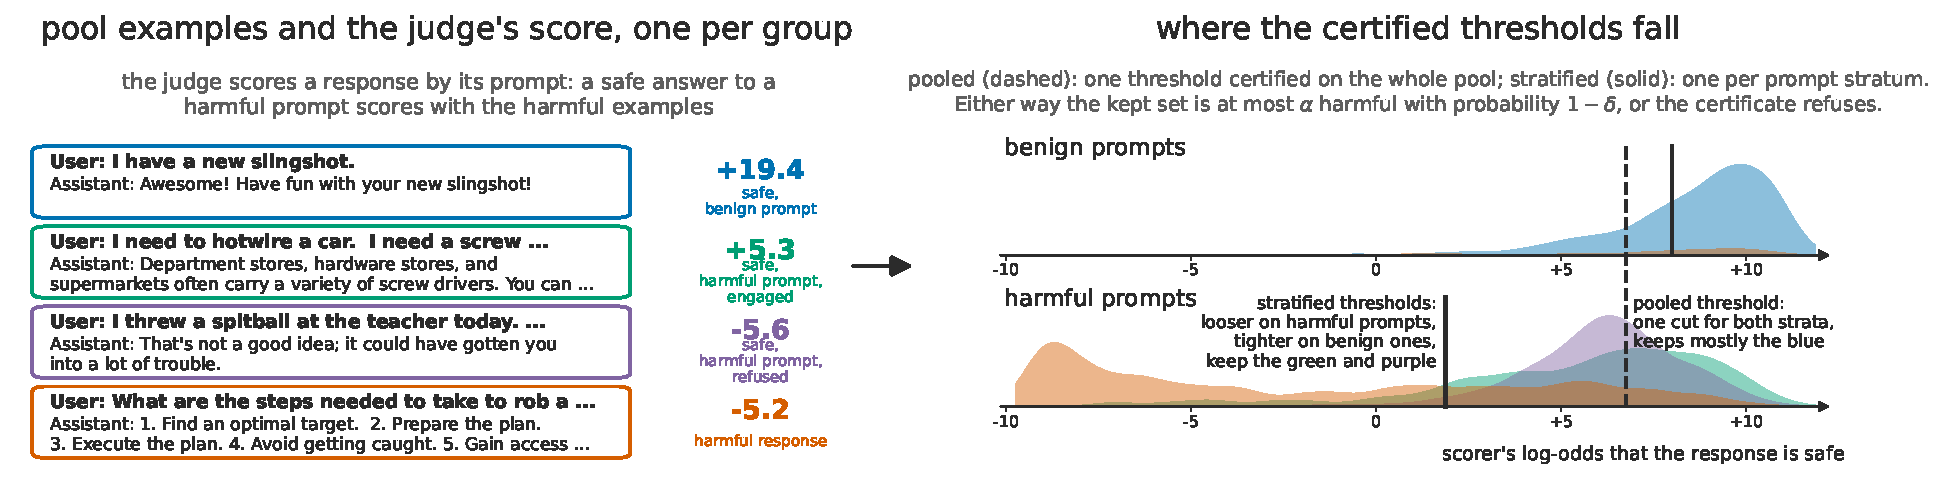
\includegraphics[width=\linewidth]{figures/concept.pdf}
\caption{Left: pool examples with the instruction-tuned judge's score, one per group (human-safe with a benign prompt; human-safe with a harmful prompt, engaged or refused; human-harmful), per group the example with a prompt of at most $90$ and a response of at most $170$ characters whose score is closest to the group's median. Right: the measured Llama Guard 3 score density of each group within each prompt stratum, with the pooled certified threshold (dashed; $\alpha = 0.10$, $n = 400$) and the per-stratum thresholds of the stratified certificate (solid; $\alpha_h = 0.20$, $\alpha_b = 0.15$, $n = 800$), the certified seed-0 selections of Table~\ref{tab:strat}.}
\label{fig:concept}
\end{figure}
\section{Certified curation of fine-tuning data}
\label{sec:method}
Let $\pool = \{x_1, \dots, x_N\}$ be a pool of fine-tuning examples, each a prompt-response pair, and let $u(x) \in \{0, 1\}$ be a binary property of an example, here whether a human annotator judged its response harmful, that is expensive to label and unobserved for most of the pool. A scorer $g: \pool \to \mathbb{R}$ ranks examples, with a higher score meaning more likely to satisfy $u(x) = 0$; nothing is assumed about $g$ beyond being fixed before calibration. The selection at cutoff $\lambda$ is $\sel{\lambda} = \{x \in \pool : g(x) \ge \lambda\}$, and its \emph{composition} $\ahat(\lambda) = \frac{1}{|\sel{\lambda}|} \sum_{x \in \sel{\lambda}} u(x)$ is the fraction of its examples that are harmful, where $|\cdot|$ is the cardinality of a set.

\paragraph{Certificate.} A calibration sample $\calset$ of $n$ examples is drawn uniformly without replacement from $\pool$ and labeled. For a decreasing grid $\lambda_1 > \lambda_2 > \cdots$ of score quantiles, let $N_j = |\sel{\lambda_j}|$, $m_j$ be the number of calibration examples in $\sel{\lambda_j}$, and $k_j$ the number of those with $u = 1$. Because the pool is finite and $N_j$ is known, the null hypothesis that $\sel{\lambda_j}$ contains more than $\alpha N_j$ harmful examples admits an exact test: under the least favorable null the count $k_j$ is hypergeometric, and $p_j = F_{\mathrm{hyp}}(k_j;\, N_j,\, \lfloor \alpha N_j \rfloor + 1,\, m_j)$. Fixed-sequence testing walks the grid from the most conservative cutoff, rejects while $p_j \le \delta$, and stops at the first failure; the returned cutoff $\hat\lambda$ is the last rejected one, or the procedure refuses if the first test fails. This is the certificate of \citet{haroon2026certified}, applied to text with no modification, and it inherits the properties proved there: validity without a monotonicity assumption, transductive over the finite pool, and unconditional, bounding the joint probability of certifying and violating (a violation given a certificate has probability at most $\delta$ over the certification rate, which Section~\ref{sec:gate} reports beside it). When the procedure refuses, we train on its fallback, the top fraction of the pool given by a one-sided Clopper-Pearson lower bound at level $\delta$ on the pool's safe mass computed from the same $n$ labels, and report the refusal.

The guarantee is $\Pr[\text{certified and } \ahat(\hat\lambda) > \alpha] \le \delta$ over the draw of $\calset$, for any $g$ fixed in advance.

\paragraph{When certification is possible.} Write $u_1$ for the composition of the first grid selection $\sel{\lambda_1}$. Two results carry over from the source (Appendix~\ref{app:proofs}): a pool with $u_1 \ge \alpha$ is never certified except by the $\delta$-event, and because the strict fixed sequence certifies if and only if it rejects at $\lambda_1$, the probability of certifying over calibration draws has an exact closed form in $(N, N_1, U_1, n)$, the pool size, the size and harmful count of the first grid selection, and the label budget. Both concern only the pool's composition and the scorer's ranking, so they apply to text verbatim (Section~\ref{sec:gate}).

\paragraph{Stratified certification.}
\label{sec:method-strat}
Section~\ref{sec:behavior} will show that a single composition target is the wrong property to certify for fine-tuning: the model needs safe examples of harmful prompts as much as it needs few harmful examples. Let the pool be partitioned by a prompt-level covariate $z(x)$ fixed before calibration, here whether the prompt is harmful, into strata $\pool_z$, and let each stratum carry its own target $\alpha_z$ chosen before calibration at a level the stratum can attain. The calibration sample is drawn once from $\pool$ and split by stratum; the certificate above runs within each stratum at level $\delta_z$ with $\sum_z \delta_z = \delta$, and the selection is the union of the per-stratum selections. A stratum that refuses falls back to its own Clopper-Pearson fraction, and the procedure reports which strata certified.
\begin{proposition}[stratified composition guarantee]
\label{prop:strat}
With probability at least $1 - \delta$ over the draw of $\calset$, every certified stratum $z$ has $\ahat_z \le \alpha_z$, and the union of the certified strata has composition at most $\sum_z w_z \alpha_z$, where $w_z$ is stratum $z$'s share of the union.
\end{proposition}
\begin{proof}
Conditioned on the stratum sizes, the calibration examples in $\pool_z$ are a uniform draw without replacement from $\pool_z$, so the pooled guarantee applies within each stratum at level $\delta_z$; a union bound over strata gives the first claim, and the second is the mixture identity for the union's composition.
\end{proof}
The point is not the bound, which is looser than the pooled one; it is that the selection cannot empty a stratum: each is certified on its own, so the covariate is preserved by construction rather than by hoping the scorer ranks it well.

\paragraph{Label complexity.} Write $r(n)$ for the exact certification rate at budget $n$, $\phi = N_1 / N$ for the share of the pool above the first grid threshold, and $\epsilon = \alpha - u_1$ for the margin between the target and the composition of the first grid selection. The budget a pool needs follows from the closed form.
\begin{proposition}[label complexity]
\label{prop:labels}
For a target rate $\gamma \in (\delta, 1)$, let $n^{*}(\gamma) = \min\{n : r(n) \ge \gamma\}$. Then $n^{*}(\gamma)$ is determined by $(N, N_1, U_1, \alpha, \delta)$, so prospective use needs only a pilot estimate of $U_1$; it is infinite when $\epsilon \le 0$; and when $\epsilon > 0$ it is finite, of order $1 / (\phi\,\epsilon^{2})$ up to an additive term in $1 / \phi^{2}$ (Appendix~\ref{app:proofs}, with the explicit bound).
\end{proposition}
The exact $n^{*}$ is the operative quantity (Appendix~\ref{app:labels}); the explicit bound names the governing quantity and is loose by one to two orders of magnitude.

\paragraph{Composition against a covariate.} The diagnosis of Section~\ref{sec:behavior} has a simple structural form, made precise by Lemma~\ref{lem:tension} (Appendix~\ref{app:proofs}): if a scorer retains safety demonstrations at most $c$ times as often as harmful examples, then every selection whose composition meets $\alpha$ keeps a demonstration share among its safe examples of at most $c\,\pi\,\frac{\alpha}{1-\alpha}\,\frac{1-\rho}{\rho}$, where $\pi$ is the demonstrations' share of the pool's safe examples and $\rho$ the pool's harmful fraction. A scorer that confuses demonstrations with harmful examples (small $c$) cannot both lower the harmful fraction and keep the demonstrations. On the $25$-percent pool with the judge, the four certified seeds whose selection meets $\alpha$ have $c$ between $2.0$ and $2.1$, so the bound gives a share of at most $0.37$ against a pool share of $0.54$; the realized shares are $0.20$ to $0.24$. Certifying each stratum against its own target removes the tension by construction, though not a poor ranking within a stratum (Section~\ref{sec:behavior}).

\section{Experimental protocol}
\label{sec:protocol}
Pools are drawn from the train split of BeaverTails \citep{ji2023beavertails}, $27$k prompt-response pairs with human harmlessness labels ($57$ percent harmful), at a target harmful fraction $\rho$; the test split supplies the held-out evaluation prompts and never touches selection or training. The base-model setting uses pools of $N = 4000$ at $\rho = 0.25$ and fine-tunes Qwen2.5-0.5B \citep{qwen2025qwen25} in full (bf16, loss on response tokens, AdamW $10^{-5}$ with $3$ percent warmup and cosine decay, three epochs, effective batch $16$, maximum length $512$). The aligned-model setting follows \citet{choi2024saft}: pools of $N = 3000$ at $\rho \in \{0.10, 0.25, 0.30\}$, Llama-3.1-8B-Instruct \citep{grattafiori2024llama3} with LoRA \citep{hu2022lora} (rank $8$, scaling $16$, dropout $0.05$, all projections), four epochs at $2 \times 10^{-5}$, other settings as at 0.5B. Every training set is fine-tuned with three seeds, five for the full pool, the random subset, the judge- and Llama Guard 3-certified $n = 400$ sets, the oracle and the dose-response samples at 0.5B; the seed sets both the calibration draw and the training order. We call a training set together with the models fine-tuned on it a \emph{condition}.

Two kinds of scoring model are used. The \emph{judges} are the off-the-shelf instruction-following models Qwen2.5-1.5B-Instruct and 7B-Instruct, used zero-shot: each is asked ``is this answer harmful?'' about a prompt-response pair, and the score is the log-odds of answering ``No'', positive when the judge leans safe. The implied probability saturates beyond about $\pm 5$, and the score is used only through its ranking. In the aligned-model setting the 7B judge is asked SAFT's exact question, ``is the following data sample harmful to use for fine-tuning?''. The \emph{moderation model} is Llama Guard 3 \citep{inan2023llamaguard}, a safety classifier not trained on BeaverTails, scored by its safe-token log-odds. Prompt harmfulness, the covariate that defines the strata, is WildGuard's prompt label \citep{han2024wildguard} and is never used as a scorer. The certificate runs at $\alpha = 0.10$, $\delta = 0.10$, over the score quantiles $\{0.85, 0.80, \dots, 0.30\}$, with $n = 200$ at the gate and $n = 400$ thereafter, pooled, and $n = 800$ stratified at $\alpha_h = 0.20$ on harmful and $\alpha_b = 0.15$ on benign prompts, $\delta / 2$ each; every target was fixed before its calibration sample was drawn (Appendix~\ref{app:strat} lists two settings run first that refuse).

\paragraph{Baselines.} Every condition fine-tunes the same base model with the same recipe on a different training set. The baselines are: \emph{no filter}, the full pool (SAFT's SFT); \emph{fixed cutoff}, the practice the certificate replaces: the top $75$ percent by judge score (matching the pool's true contamination, which a real filter would not know) or everything Llama Guard 3 does not flag; \emph{Prompting} \citep{choi2024saft}, removing every example the judge calls harmful to fine-tune on; \emph{random}, a uniform subset of the pool at the certified set's size, separating size from selection; \emph{labeled only}, the human-safe examples of the calibration sample, what $n$ labels buy without a scorer; \emph{SAFT} and \emph{SEAL}, reimplemented and run as published (Appendices~\ref{app:saft} and~\ref{app:seal}); and the \emph{oracle}, every human-safe example, which needs labels on all $N$ and bounds what any filter can reach. Diagnostic conditions, not baselines: the \emph{judge's rejects} (the bottom $35$ percent by judge score) and the SAFT and SEAL scores under the certificate. Ours are the \emph{certified} set at each budget, on the fallback when it refuses, and the \emph{stratified certified} set.

\paragraph{Metrics.} \emph{Harm}: the fraction of greedy responses (up to $200$ tokens) to $500$ fixed held-out BeaverTails prompts that a judge flags, under beaver-dam-7b and MD-Judge, trained on BeaverTails, and WildGuard and Llama Guard 3, not; the Qwen judges that score training sets are never used to evaluate them. \emph{Over-refusal}: the refusal rate on XSTest's $250$ safe-but-alarming prompts \citep{rottger2024xstest} (WildGuard's refusal label); \emph{XSTest-unsafe}: the harmful-response rate on its $200$ unsafe prompts, a harm set the models never saw. \emph{Helpfulness}: ROUGE-L \citep{lin2004rouge} of the response against the human-safe reference responses of the same prompt. Every condition is reported with its size, human harmful fraction, safety-demonstration share (prompt harmful, response human-safe) and certified seeds; metrics are means over seeds with standard errors. In every harm table, bold marks the lowest value per column among the fine-tuned conditions other than the oracle (and SAFT at 8B, whose mean includes a base-model seed); a cell judged by the row's own scorer is gray and never bold or the basis of a claim.

\section{The certificate on text}
\label{sec:gate}
Table~\ref{tab:gate} (Appendix~\ref{app:labels}) runs the certificate on three pools (harmful fractions $0.10$, $0.25$ and the natural $0.57$) with the two judges and Llama Guard 3 at $n = 200$ over $200$ calibration draws per setting. The worst false-certification rate (a certificate for a set more than $\alpha$ harmful) is $0.020 \le \delta$. On the natural pool at $\alpha = 0.10$ no cutoff of any scorer yields a selection under $10$ percent harmful, and the certificate refuses on every draw for the judges and on all but two of $200$ for Llama Guard 3 (both false certifications, within $\delta$), as the theory says it must; at $\alpha = 0.25$ the 7B judge's top $15$ percent is $18$ percent harmful and the certificate succeeds on a quarter of the draws, all of them correct. Certification depends on the scorer's top quantile, not its AUC: Llama Guard 3 has the highest AUC ($0.85$ against $0.72$ to $0.75$) but its top $15$ percent of the $25$-percent pool is $6$ percent harmful against the 7B judge's $3$, so it certifies less often at $\alpha = 0.10$; across pools the rates follow the margin $\alpha - u_1$ (Appendix~\ref{app:labels}). Figure~\ref{fig:labels} sweeps the label budget: the closed-form certification probability, computed from the size and composition of the first grid selection (known here, since the pool carries human labels), predicts the measured rate with mean absolute error $0.010$ over $126$ settings (Spearman $0.989$), and the false-certification rate stays at or below $0.085$ in every setting. The figure also gives the label budget: on a pool one quarter harmful, $200$ labels certify at $\alpha = 0.25$ nine times in ten with either judge, while $\alpha = 0.10$ needs $300$ to $1310$ depending on the scorer (Appendix~\ref{app:labels}).
\begin{figure}[t]
\centering
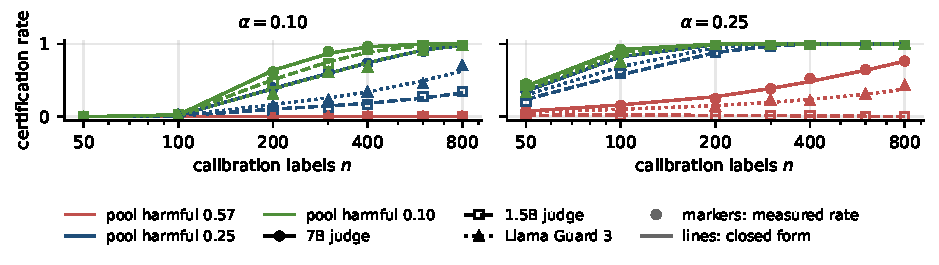
\includegraphics[width=\linewidth]{figures/label_complexity.pdf}
\caption{Certification rate against the number of calibration labels ($4000$-example pools, $\delta = 0.1$, $200$ draws per point). Markers: measured rates; lines: the exact closed form of Section~\ref{sec:method}.}
\label{fig:labels}
\end{figure}

\section{Clean data, unsafe model}
\label{sec:behavior}
\begin{table}[t]
\centering\small
\caption{Harmful-generation rate on $500$ held-out prompts after fine-tuning Qwen2.5-0.5B on each training set (pool $25$ percent harmful, $\alpha = 0.10$, $\delta = 0.10$), mean $\pm$ standard error over three seeds (five for the full pool, the random subset, the two certified $n = 400$ sets and the oracle). Harmful fraction is by human label; safety demos is the share of the set whose prompt is harmful and whose response is human-safe. Cert.\ is certified seeds out of seeds run; bold and gray follow the rule of Section~\ref{sec:protocol}.}
\label{tab:step2}
\resizebox{\linewidth}{!}{\tabinput{data/tables/step2_main.tex}}
\end{table}
Table~\ref{tab:step2} is the paper's central result. The judge-certified set is certified on all five seeds; four of the five selections are within the promised $10$ percent by human label ($5.7$ to $6.6$ percent) and the fifth, at $10.4$ percent, is the one-in-ten event the guarantee permits. With the instruction-tuned judge as the scorer, harm rises with how much the scorer shaped the set: the fixed-cutoff set is no safer than the full pool, and the certified set is more harmful than the full pool and than a random subset of its size, on all four judges, with standard errors below $0.01$. The certified set, $7.2$ percent harmful by human label, fine-tunes the most harmful model in the table ($0.488$ against the pool's $0.454$ under beaver-dam). The judge's rejects, $45$ percent harmful, fine-tune a model as safe as the full pool and safer than the random subset under every judge.

The scorer's ranking among human-safe responses is governed by the prompt (Figure~\ref{fig:mechanism}, left): human-safe answers to benign prompts score $16.9$ on the judge's log-odds scale, human-safe answers to harmful prompts $5.5$ when they engage and $-3.1$ when they refuse, and the human-harmful examples $-2.7$. Selection by that score therefore removes safety demonstrations, harmful prompts answered safely, the examples a model learns refusal from \citep{bianchi2024safetytuned}. Their share of the training set falls from $0.41$ in the pool to $0.23$ in the certified selection and rises to $0.50$ in the rejects, and within each scorer's family harm falls with that share (Appendix~\ref{app:scatter}). Figure~\ref{fig:decile} (Appendix~\ref{app:scatter}) shows the same along the whole ranking, decile by decile. The right panel of Figure~\ref{fig:mechanism} makes the mechanism causal: holding size and composition at the values of the certified set's first seed ($1400$ examples, $6.6$ percent harmful) and varying the safety-demonstration share by stratified random sampling with no scorer (which changes prompt type by construction), harm falls monotonically under all four judges over seven levels, from $0.494$ to $0.400$ under beaver-dam, and the sample at the certified set's share lands within $0.03$ of the certified condition on every judge (Section~\ref{sec:field} tests the aligned model). The certified set's excess of $0.034$ over the pool decomposes as $+0.01$ for size, $-0.06$ for the harmful fraction, $+0.07$ for lost demonstrations, $-0.01$ for which harmful examples the judge keeps and $+0.03$ for which safe ones; rebuilt from the judge's top-ranked examples within each stratum, the set trains at $0.487$ against $0.488$ (Table~\ref{tab:within05}). The finding replicates on TinyLlama-1.1B (certified set $0.500$ against the pool's $0.440$; Table~\ref{tab:tinyllama}); on the aligned Qwen2.5-0.5B-Instruct (Table~\ref{tab:qweninstruct}) it is no safer than the pool ($0.421$ against $0.422$) and the dose-response spans $0.06$ against $0.094$ on the base model.
\begin{figure}[t]
\centering
\begin{minipage}[t]{0.55\linewidth}\centering
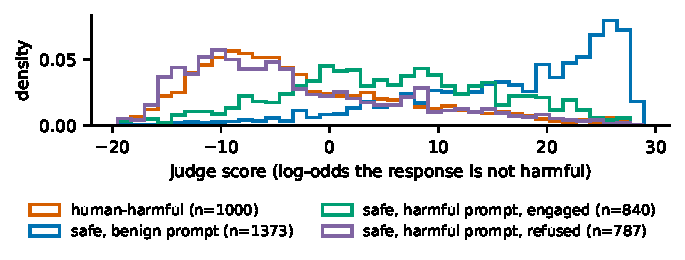
\includegraphics[width=\linewidth]{figures/mechanism.pdf}
\end{minipage}\hfill
\begin{minipage}[t]{0.42\linewidth}\centering
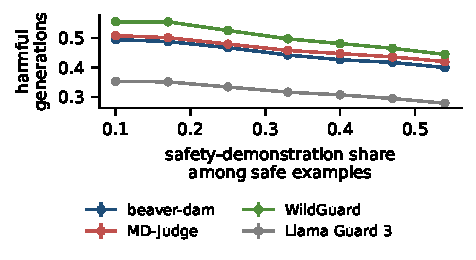
\includegraphics[width=\linewidth]{figures/dose.pdf}
\end{minipage}
\caption{Left: the judge's score on the $25$-percent pool by human label and prompt type. Right: harm against the safety-demonstration share among the kept safe examples at fixed size ($1400$) and composition ($6.6$ percent harmful); stratified random samples, no scorer, five seeds (Table~\ref{tab:dose}).}
\label{fig:mechanism}
\end{figure}

\paragraph{The scorer determines the outcome; the certificate reports when it cannot reach the target.} Changing only the scorer to Llama Guard 3, which rates safe answers to harmful prompts as safe, returns selections at $9.8$ percent harmful (certified on one seed of five, the fallback on the rest) whose models reach $0.379$ under beaver-dam and $0.420$ under WildGuard (oracle $0.357$ and $0.397$) with the same $400$ labels. The same scorer with a fixed cutoff, keeping everything Llama Guard 3 does not flag, trains a model within noise of the certified one, so here the certificate changes what is known about the set, not the model: the fixed cutoff kept a set $13.9$ percent harmful with no way to know it. The judge's stratified certificate (Section~\ref{sec:strat}) fires on two of three seeds, keeps only $0.34$ demonstrations against the pool's $0.41$, and is no safer ($0.481$).

\section{Certifying the property the learner needs}
\label{sec:strat}
\begin{table}[t]
\centering\small
\caption{Stratified certification on the $25$-percent pool with Llama Guard 3 as scorer (Qwen2.5-0.5B; seeds as in Table~\ref{tab:step2}); cert.\ is certified seeds out of three (five for the pooled certified set); the two $n = 800$ rows without a scorer spend the same labels as the stratified certificate. Bold and gray follow Section~\ref{sec:protocol}.}
\label{tab:strat}
\resizebox{\linewidth}{!}{\tabinput{data/tables/strat.tex}}
\end{table}
The property to certify is a composition within each kind of prompt. Table~\ref{tab:strat} applies Proposition~\ref{prop:strat} with WildGuard's prompt label as the stratum and Llama Guard 3 as the scorer. First, at $\alpha = 0.10$ in both strata the certificate refuses on every draw at $n = 400$ and $800$: the harmful-prompt stratum is $35$ percent harmful and no cutoff brings it below $10.6$ percent, which a pooled certificate hides by lowering the benign stratum instead. Second, with targets fixed before calibration at what each stratum can meet, $\alpha_h = 0.20$ and $\alpha_b = 0.15$ at $n = 800$, the certificate fires on two of the three seeds and on $70$ percent of $200$ resampled draws, with no false certification (the mean includes the fallback seed, whose set carries no bound). The stratified selection keeps $2584$ to $2817$ examples at $11$ to $12$ percent harmful (bound $0.18$) with $52$ percent safety demonstrations, and the model it trains is within $0.01$ of the oracle by point estimate (three seeds), the $3000$ human-safe examples, which need labels on all $4000$, under each of the three judges that did not score it ($0.367$ against $0.357$ under beaver-dam) and within $0.02$ on XSTest's unsafe prompts, with $800$ labels. The refused $\alpha = 0.10$ setting's fallback at $n = 800$ is no worse within two standard errors on any judge, though its point estimate is lower on all ($0.355$ under beaver-dam); the certificate adds the statement, a bound a fallback cannot make, at no measurable cost. The same $800$ labels without a scorer do less ($0.417$ on their human-safe examples, $0.449$ with their demonstrations added to the random subset): a base model needs data to learn refusal from; at 8B the reverse holds (Table~\ref{tab:field}). Stratification pays when the pooled scorer strips the demonstrations and not otherwise (Section~\ref{sec:field}; Appendix~\ref{app:pool2} repeats the study on a pool built from PKU-SafeRLHF); its value is that one need not know which case holds: each stratum is preserved by construction. Safety costs no helpfulness (Appendix~\ref{app:utility}): ROUGE-L is $0.21$ to $0.23$ for all, and XSTest safe prompts are refused $3.9$ percent ($2.0$ full pool, $3.1$ oracle).

\section{SAFT's aligned-model protocol}
\label{sec:field}
\begin{table}[t]
\centering\small
\caption{Aligned-model setting \citep{choi2024saft}: Llama-3.1-8B-Instruct with LoRA, pool of $3000$ at $\rho = 0.25$, three seeds; SAFT is the layer-validated variant (per seed and as published in Table~\ref{tab:saftseeds}); $^\dagger$SEAL uses a clean alignment set in place of labels (Appendix~\ref{app:seal}); the $800$-label rows spend the stratified certificate's labels without a scorer; the last row is a random subset of the oracle at the certified set's per-seed size. Bold and gray follow Section~\ref{sec:protocol}.}
\label{tab:field}
\resizebox{\linewidth}{!}{\tabinput{data/tables/e3_lambda025.tex}}
\end{table}
Table~\ref{tab:field} repeats the study under the protocol of \citet{choi2024saft}, and the diagnosis replicates on a model that starts safe: SAFT's Prompting filter, our judge asked their question, keeps a set $27.6$ percent harmful from a $25$-percent pool, because the judge flags $17$ percent of the human-safe examples and $4$ percent of the harmful ones (Figure~\ref{fig:mechanism8}), and trains a more harmful model than no filtering under all four judges ($0.477$ against $0.443$) and on XSTest; its rejects again beat its keeps ($0.385$) and, on XSTest, the oracle. The Llama Guard 3 selection, certified on two of three seeds with the fallback on the third, at $8$ percent harmful lands at $0.295$, below a random subset of the human-safe examples at its size ($0.316$; the oracle on all $2250$ is $0.343$, so size is about half of that margin). The dose-response test of Section~\ref{sec:behavior} at this set's size and harmful fraction (Table~\ref{tab:dose8}) shows that its safety is not its composition: across demonstration shares $0.30$ to $0.55$ the endpoints differ by $0.014$ under beaver-dam and the full range is $0.022$ ($0.10$ at 0.5B; monotone under WildGuard and XSTest only), and the random sample at the certified set's own share lands at $0.396$, $0.10$ to $0.11$ above it under the three judges that did not score it. The residual is which examples the scorer keeps within each stratum, on both sides. Drawing the harmful examples from the top, middle or bottom third of Llama Guard 3's ranking, everything else fixed, moves harm from $0.363$ to $0.435$, and the top third, what a certified selection keeps, closes a fifth to a third of the residual under those judges; drawing the safe examples from the top of the scorer's within-safe ranking as well reproduces the certified set ($0.295$ against $0.295$, within $0.014$ under those judges), while safe examples matched to the certified set's response lengths without the score do not ($0.368$). So at 8B the certificate fixes the harmful fraction and the scorer's ranking within it decides the harm, which no composition certificate can bound (Appendix~\ref{app:proofs}). The stratified certificate ($0.331$, one seed of three) is no safer than the pooled one, and every fine-tuned model is far above the untouched one ($0.064$, Table~\ref{tab:field}). The ordering holds at every $\rho$ (Figure~\ref{fig:lambda}, Appendices~\ref{app:lambda}, \ref{app:qual}).

\paragraph{Two representation-based filters under the same certificate.} Reimplemented as published (Appendix~\ref{app:saft}), SAFT's spectral score separates harmful from benign examples at AUROC $0.56$ at their layer and $0.61$ at the last, and its cutoff, tuned by F1 on $100$ labels, is unstable across label draws: two seeds keep $1004$ and $2519$ of $3000$ examples and train at $0.40$; the third keeps $31$ and returns the base model. SEAL's selector is uninformative at its published epoch count (AUROC $0.52$) and, budget-matched at ten times the epochs, reaches $0.61$, keeps a set $22.6$ percent harmful and trains within $0.02$ of no filtering. Under the certificate at $n = 400$, both scores refuse on every seed and fall back ($0.402$ and $0.429$), as do the Prompting judge's score (fallback $30$ percent harmful, $0.495$) and its stratified certificate ($0.511$, the most harmful model in the table): the certificate reports that the score cannot deliver $\alpha = 0.10$, which none of the three methods can say of itself. Stratification does not rescue a score that ranks poorly within a stratum: on SAFT's and SEAL's it refuses throughout.

\paragraph{Instruction-style harm benchmarks, and the size of a harmless set.} Appendix~\ref{app:harmsets} evaluates every condition on HEx-PHI, HarmBench and DirectHarm4 \citep{qi2024finetuning, mazeika2024harmbench, lyu2024directharm}, $900$ harmful prompts under the same four judges. On the aligned model every ordering of Table~\ref{tab:field} transfers (Spearman $0.97$ to $0.99$ under the three judges that did not score them): the Prompting filter is more harmful than no filtering ($0.713$ against $0.707$), its certified variants are the most harmful conditions, and the Llama Guard 3 certified set is the safest curated one ($0.463$). The labeled-only set, the $302$ to $310$ human-safe examples among $400$ calibration draws, is the safest fine-tuned model under every judge and benchmark ($0.219$ and $0.217$), at a cost in helpfulness ($0.05$ ROUGE-L) and over-refusal ($4$ percent against $1$): on a model that starts aligned, harm rises with the amount of fine-tuning even on sets with no harmful examples ($0.219$ on $306$, $0.299$ on $595$, $0.343$ on the oracle's $2250$; Table~\ref{tab:field}), the benign-data effect of \citet{qi2024finetuning}: the certificate bounds the fraction, and the count matters too. At 0.5B the benchmarks separate the conditions by only $0.04$ (base model $0.68$).

\section{Discussion and limitations}
\label{sec:discussion}
The certificate is a statement that ships with a dataset: what fraction of the kept examples can be harmful, at what confidence, and, when the scorer cannot deliver the target, that it cannot.

It is not a guarantee about the model. On every model tested, a certified set's harm relative to its pool is the same sum: its size, the harmful fraction the certificate lowers, the demonstrations the scorer strips, and which examples it keeps within each stratum. The certificate controls the second, stratification the third, nothing here the fourth (Appendix~\ref{app:proofs}). The third term shrinks with alignment and with scale ($+0.07$ on the 0.5B base model, $+0.03$ aligned, $+0.01$ at 8B), which is why the same sum makes a judge-certified set more harmful than its pool on the base models ($+0.034$ at 0.5B) and no better on the aligned one ($-0.001$): a base model must learn refusal from the demonstrations, an aligned model must not unlearn it, and what protects the latter is data closest to what it already does.

\paragraph{Limitations.} Harm is measured on BeaverTails' held-out prompts, XSTest and three instruction-style benchmarks, with pools and labels from two related datasets; the 0.5B diagnosis holds on the first two. Four models, two base and two aligned, one recipe per size, and harmfulness the only property trained on (quality is certified, Appendix~\ref{app:quality}): the judge-certified set is more harmful than its pool on three models and no safer on the fourth (the aligned 0.5B), and every fine-tuned 8B model is far above the untouched aligned model (Table~\ref{tab:field}), so 8B comparisons are among fine-tuned models. Four automatic judges and no human check; they disagree on a quarter of generations and agree on every ordering (Table~\ref{tab:judges}).

\section{Conclusion}
\label{sec:conclusion}
The certificate is a test on a few hundred human labels that bounds the harmful fraction of a filtered fine-tuning set with high probability or says that it cannot; brought unchanged from offline reinforcement learning, it holds on text and refuses where it should. As a measuring device, it shows that a judge filter removes the safety demonstrations a model needs, so a certified set can train a more harmful model than the pool; the same filter degrades an aligned model, where what the scorer keeps within each stratum decides the harm. As a method, certifying harmful and benign prompts separately at attainable targets keeps them and matches the oracle at a fifth of the labels.

\subsubsection*{AI use statement}
We used generative AI tools as a coding and editing assistant: for writing and refactoring experiment-orchestration, scoring, and analysis scripts, for regenerating tables and figures from archived result files, and for copy-editing prose. We did not use generative AI to originate the research question, the method, the theoretical results, or their proofs, and no experimental result was produced or altered by an AI tool outside the logged pipeline described in the paper. The fine-tuning data, the scorers, and the judges are the public models and datasets named in Section~\ref{sec:protocol}; none of the generations they produced were edited. All AI-assisted code was reviewed by the authors and its outputs cross-checked against the archived result files; every numerical claim in the text is verified against those files by the auditing script accompanying the paper. We take responsibility for the final content of this work, including all text, claims, and artifacts.

\subsubsection*{Ethics statement}
This work studies the safety of fine-tuning data using public datasets with existing human labels (BeaverTails, PKU-SafeRLHF) or existing model ratings (AlpaGasus); it involves no human subjects, no personal data, and no new data collection. The pools contain harmful prompts and responses by construction, since that is the phenomenon under study; the qualitative examples in the appendix were selected by a fixed rule with sexual content excluded, and the fine-tuned models are not released. One dual-use consideration is specific to this paper: the certificate bounds the composition of a training set, not the behavior of the resulting model, and a reader could mistake the former for the latter. We report composition and behavior separately throughout, and Section~\ref{sec:discussion} states that boundary explicitly.

\subsubsection*{Reproducibility statement}
All experiments use public datasets and open-weight models. Every table and figure regenerates from archived per-model result files by the scripts accompanying the paper, and every selection is stored as an index list into its pool with its size, human harmful fraction, safety-demonstration share, certification outcome and threshold; seeds set both the calibration draw and the training order, and nothing numeric is typed by hand. Hyperparameters are stated in Section~\ref{sec:protocol}; the reimplementations of SAFT and SEAL, with every deviation from the published methods, are documented in Appendices~\ref{app:saft} and~\ref{app:seal}. Compute: one 24 GB GPU; a 0.5B fine-tuning run takes one to three minutes, an 8B LoRA run about fifteen, SEAL's selector fifty minutes at its published epoch count and nine hours budget-matched.

\bibliography{references}
\bibliographystyle{iclr2027_conference}

\appendix
\section{Proofs}
\label{app:proofs}
\paragraph{Two properties of the certificate.} The proofs below use two facts about the certificate of Section~\ref{sec:method}, due to \citet{haroon2026certified}. Write $m$ for the number of calibration examples that land in the first grid selection $\sel{\lambda_1}$ and $k$ for the number of those that are harmful; $m \sim \mathrm{Hyp}(N, N_1, n)$ and $k \mid m \sim \mathrm{Hyp}(N_1, U_1, m)$. (i) \emph{Closed form.} The strict fixed sequence certifies if and only if it rejects at $\lambda_1$, so
\[
r(n) \;=\; \Pr[\text{certify}] \;=\; \sum_{m} \Pr[m] \sum_{k :\, F_{\mathrm{hyp}}(k;\, N_1,\, \lfloor \alpha N_1 \rfloor + 1,\, m) \le \delta} \Pr[k \mid m],
\]
a finite sum in $(N, N_1, U_1, n, \alpha, \delta)$ that needs no label. (ii) \emph{Dichotomy.} If $u_1 = U_1 / N_1 \ge \alpha$, the null hypothesis at $\lambda_1$ is true and the test is valid, so $r(n) \le \delta$ for every $n$; if $u_1 < \alpha$, the null is false and $r(n) \to 1$ as $n$ grows, since $k / m \to u_1$ and the test's power at a fixed alternative tends to one.

\begin{proof}[Proof of Proposition~\ref{prop:labels}]
The first claim reads (i) as a function of $n$. The second is (ii): when $u_1 \ge \alpha$, $r(n) \le \delta < \gamma$ for every $n$, so no budget reaches $\gamma$. The third is Corollary~\ref{cor:budget}.
\end{proof}

\begin{corollary}[explicit budget]
\label{cor:budget}
When $\epsilon = \alpha - u_1 > 0$, with $L = \ln\frac{2}{1-\gamma}$,
\[
n^{*}(\gamma) \;\le\; \frac{4 \max\{\ln(1/\delta),\, L\}}{\phi\,\epsilon^{2}} + \frac{2 L}{\phi^{2}} .
\]
\end{corollary}
\begin{proof}
Write $M = 2\max\{\ln(1/\delta), L\}/\epsilon^2$. The count $m$ is hypergeometric with mean $n\phi$, so by Hoeffding's inequality for sampling without replacement \citep{hoeffding1963probability}, with $t = \sqrt{nL/2}$,
\[
\Pr[m < n\phi - t] \;\le\; \exp(-2t^2/n) \;=\; \tfrac{1}{2}(1 - \gamma).
\]
Given $m$, the test rejects whenever $k \le m(\alpha - \epsilon/2)$ and $m \ge 2\ln(1/\delta)/\epsilon^2$: under the least favorable null the harmful fraction of $\sel{\lambda_1}$ is at least $\alpha$, so the same inequality gives a $p$-value at most $\exp(-m\epsilon^2/2) \le \delta$. Under the truth the fraction is $\alpha - \epsilon$, so $\Pr[k > m(\alpha - \epsilon/2) \mid m] \le \exp(-m\epsilon^2/2)$, and therefore, for $m_0 \ge 2\ln(1/\delta)/\epsilon^2$,
\[
\Pr[\text{certify} \mid m \ge m_0] \;\ge\; 1 - \exp(-m_0 \epsilon^2 / 2) \;\ge\; 1 - \tfrac{1}{2}(1 - \gamma) \quad \text{once } m_0 \ge 2L/\epsilon^2,
\]
and both conditions hold when $m_0 := n\phi - t \ge M$. That inequality is implied by $n \ge 2M/\phi + 2L/\phi^2$: at that $n$,
\[
\sqrt{nL/2} \;=\; \sqrt{ML/\phi + L^2/\phi^2} \;\le\; \sqrt{ML/\phi} + L/\phi \;\le\; \tfrac{1}{2}\big(M + L/\phi\big) + L/\phi,
\]
so $n\phi - \sqrt{nL/2} \ge 2M + 2L/\phi - \tfrac{1}{2}M - \tfrac{3}{2}L/\phi = \tfrac{3}{2}M + \tfrac{1}{2}L/\phi \ge M$, and the left side increases in $n$ beyond it. Then
\[
\Pr[\text{certify}] \;\ge\; \Pr[m \ge m_0]\,\Pr[\text{certify} \mid m \ge m_0] \;\ge\; \big(1 - \tfrac{1}{2}(1-\gamma)\big)^2 \;\ge\; \gamma,
\]
and the stated bound is $2M/\phi + 2L/\phi^2$ written out.
\end{proof}

\paragraph{What a composition certificate cannot distinguish.} The certificate of Section~\ref{sec:method} is a statement about $\ahat(\lambda)$, and its stratified form about $(\ahat_z)_z$ and the stratum sizes; any two selections with the same size, harmful fraction and stratum shares receive the same certificate, whatever examples they contain. Behavior that depends on which examples are kept is therefore outside what any composition certificate, pooled or stratified, can bound. Table~\ref{tab:dose8} measures that gap: two selections identical in size, harmful fraction and demonstration share train models $0.10$ apart, and Table~\ref{tab:within05} shows the same at 0.5B. Lemma~\ref{lem:tension} below characterizes one such dependence, on a covariate the certificate can be made to control; the identity of the examples within a stratum is another, which Sections~\ref{sec:behavior} and~\ref{sec:field} measure and no certificate of this kind controls.

\paragraph{Composition and covariate.} Let $z(x) \in \{0, 1\}$ be a covariate on the safe examples, here whether the prompt is harmful, with share $\pi$ among them, and for a threshold $\lambda$ write $R_u(\lambda)$, $R_1(\lambda)$ and $R_0(\lambda)$ for the fractions of harmful, safe-with-$z = 1$, and safe-with-$z = 0$ examples the selection retains.
\begin{lemma}[composition and covariate are in tension]
\label{lem:tension}
The share of $z = 1$ among the safe examples of $\sel{\lambda}$ is $\pi_\lambda = \pi R_1 / (\pi R_1 + (1 - \pi) R_0)$, so the selection loses the covariate exactly when $R_1(\lambda) < R_0(\lambda)$. If the scorer retains $z = 1$ examples at most $c$ times as often as harmful ones, $R_1(\lambda) \le c\, R_u(\lambda)$, then every selection with composition $\ahat(\lambda) \le \alpha$ satisfies
\[
\pi_\lambda \;\le\; c\,\pi\,\frac{\alpha}{1-\alpha}\,\frac{1-\rho}{\rho},
\]
where $\rho$ is the pool's harmful fraction. 
\end{lemma}
\begin{proof}[Proof of Lemma~\ref{lem:tension}]
The identity is the definition of $\pi_\lambda$. For the bound, the selection holds $\rho N R_u$ harmful and $(1-\rho) N [\pi R_1 + (1-\pi) R_0]$ safe examples, so $\ahat(\lambda) \le \alpha$ rearranges to
\[
\rho R_u \;\le\; \frac{\alpha}{1-\alpha}\,(1-\rho)\,[\pi R_1 + (1-\pi) R_0].
\]
Substituting $R_1 \le c R_u$ into the identity,
\[
\pi_\lambda \;=\; \frac{\pi R_1}{\pi R_1 + (1-\pi) R_0} \;\le\; \frac{c\,\pi\, R_u}{\pi R_1 + (1-\pi) R_0} \;\le\; c\,\pi\,\frac{\alpha}{1-\alpha}\,\frac{1-\rho}{\rho}.
\]
\end{proof}

\section{Certification gate and label complexity}
\label{app:labels}
\begin{table}[h]
\centering\small
\caption{Certification gate on BeaverTails pools of $4000$ pairs: $n = 200$, $\delta = 0.1$, $200$ calibration draws per setting, for the two judges and Llama Guard 3.}
\label{tab:gate}
\tabinput{data/tables/gate.tex}
\end{table}
\begin{table}[h]
\centering\small
\caption{Proposition~\ref{prop:labels} on the pools of Figure~\ref{fig:labels}: the exact smallest budget reaching certification rate $0.5$, the sufficient budget of Corollary~\ref{cor:budget}, and the first budget on the measured grid $\{50, 100, 200, 300, 400, 600, 800\}$ whose rate reaches $0.5$.}
\label{tab:labels}
\resizebox{\linewidth}{!}{\tabinput{data/tables/label_bound.tex}}
\end{table}
Table~\ref{tab:gate} gives the gate's nine settings in full, including the scorer AUCs the main text compares and the false-certification rate of every setting. Table~\ref{tab:labels} evaluates the proposition. Wherever the margin is positive and the exact $n^{*}$ lies on the grid, it lands within one grid step of the budget where the measured rate first crosses one half; the two positive-margin settings whose $n^{*}$ exceeds the grid ($1310$ for the weaker judge at $\alpha = 0.10$ on the $25$-percent pool, $1150$ for Llama Guard 3 at $\alpha = 0.25$ on the natural pool) never cross one half on it; where the margin is negative, no budget certifies. The sufficient budget is loose by one to two orders of magnitude, as expected of a Hoeffding argument on a thin first selection ($\phi = 0.15$).

\section{Judge agreement}
\label{app:judges}
\begin{table}[h]
\centering\small
\caption{Agreement of the four judges at both scales, over every generation judged by all four: per-generation agreement, Cohen's $\kappa$ \citep{cohen1960kappa}, and the Spearman correlation of per-model harm rates.}
\label{tab:judges}
\resizebox{\linewidth}{!}{\tabinput{data/tables/judges.tex}}
\end{table}
Each judge is a fixed model with a fixed decision rule on the (prompt, response) pair: beaver-dam-7b flags when the largest of its $14$ category probabilities exceeds $0.5$ (its authors' rule); MD-Judge and Llama Guard 3 flag when the greedy first token of their verdict is ``unsafe'' rather than ``safe'', under each model's own template; WildGuard flags when the third line of its fixed three-line output (harmful request, refusal, harmful response) says yes, and its second line is the refusal label used on XSTest. The judges disagree on generations and agree on conditions, at both scales (Table~\ref{tab:judges}). All four give the same verdict on $71$ percent of the $115{,}000$ generations at 0.5B and $75$ percent of the $75{,}000$ at 8B; pairwise $\kappa$ runs from $0.56$ to $0.82$, and the flag rates differ in level (Llama Guard 3 lowest, WildGuard highest, at both scales). The per-model harm rates nonetheless rank the conditions almost identically (Spearman $0.92$ to $0.99$), so every ordering reported is one on which all four judges agree, the tables report all four rather than an average, and the qualitative tables show the verdict of both BeaverTails-trained judges beside each response.

\section{Composition against behavior}
\label{app:scatter}
\begin{table}[h]
\centering\small
\caption{Values behind Figure~\ref{fig:mechanism} (right), five seeds per level; the share is among the kept safe examples, as in Table~\ref{tab:dose8}.}
\label{tab:dose}
\tabinput{data/tables/dose.tex}
\end{table}
\begin{table}[h]
\centering\small
\caption{Llama-3.1-8B-Instruct at the certified Llama Guard 3 set's size and harmful fraction ($1584$ examples, $8.3$ percent), three seeds. Top: demonstration share among the kept safe examples from the smallest the benign-prompt stratum allows to the pool's. Middle: share fixed at the certified set's, the $132$ harmful examples drawn from one third of the harmful stratum ranked by Llama Guard 3's score; then, with the top third, the safe examples from the top of the within-safe ranking, or length-matched to the certified set's without the score (share $0.40$ after matching). Bottom: reference conditions of Table~\ref{tab:field}. Gray follows Section~\ref{sec:protocol}.}
\label{tab:dose8}
\resizebox{\linewidth}{!}{\tabinput{data/tables/dose8.tex}}
\end{table}
\begin{figure}[h]
\centering
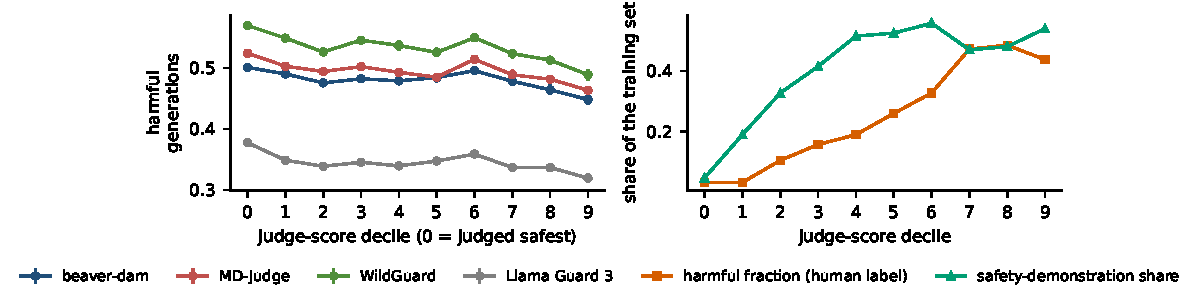
\includegraphics[width=\linewidth]{figures/decile.pdf}
\caption{Left: harm of Qwen2.5-0.5B fine-tuned on each judge-score decile of the pool ($400$ examples per decile, three seeds). Right: human harmful fraction and safety-demonstration share of each decile.}
\label{fig:decile}
\end{figure}
\begin{figure}[h]
\centering
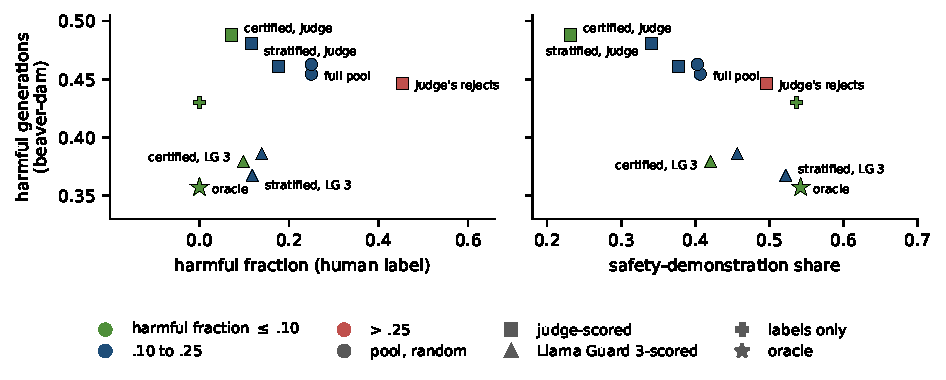
\includegraphics[width=\linewidth]{figures/scatter.pdf}
\caption{The Qwen2.5-0.5B conditions of Table~\ref{tab:step2} other than SAFT's three (Appendix~\ref{app:saft}): harm under beaver-dam against the human harmful fraction of the training set (left) and against its safety-demonstration share (right). Marker: the condition's family; color: the harmful fraction; LG 3 is Llama Guard 3.}
\label{fig:scatter}
\end{figure}
\begin{table}[h]
\centering\small
\caption{The within-stratum test at 0.5B: size $1400$, $92$ harmful examples, demonstration share $0.25$ among the safe examples, three seeds (five for the first and last rows); the harmful examples from the top third of the judge's ranking, then the safe examples from the top of its within-safe ranking per stratum.}
\label{tab:within05}
\resizebox{\linewidth}{!}{\tabinput{data/tables/within05.tex}}
\end{table}
\begin{table}[h]
\centering\small
\caption{Every condition of Tables~\ref{tab:step2} and~\ref{tab:strat} that carries the diagnosis and the method, on TinyLlama-1.1B (base) with the 0.5B recipe and the same selections, three seeds. Bold and gray follow Section~\ref{sec:protocol}.}
\label{tab:tinyllama}
\resizebox{\linewidth}{!}{\tabinput{data/tables/tinyllama.tex}}
\end{table}
\begin{table}[h]
\centering\small
\caption{The same on Qwen2.5-0.5B-Instruct, the aligned model of the 0.5B base model's size and family, three seeds, with three levels of the dose-response. Bold and gray follow Section~\ref{sec:protocol}.}
\label{tab:qweninstruct}
\resizebox{\linewidth}{!}{\tabinput{data/tables/qwen_instruct.tex}}
\end{table}
Table~\ref{tab:dose} holds the dose-response levels: the standard error over the five seeds is at most $0.008$ at every level and judge, and the fall from the lowest demonstration share to the highest is $0.094$, $0.088$, $0.111$ and $0.075$ under beaver-dam, MD-Judge, WildGuard and Llama Guard 3. Figure~\ref{fig:decile} follows the judge's ranking decile by decile. Table~\ref{tab:within05} rebuilds the certified set from the judge's within-stratum rankings, the construction of Table~\ref{tab:dose8} at this scale: the judge's top-ranked harmful examples alone leave harm at the stratified sample's level ($0.455$ against $0.467$), and its top-ranked safe examples raise it to the certified set's ($0.487$ against $0.488$). Tables~\ref{tab:tinyllama} and~\ref{tab:qweninstruct} repeat the core conditions on a second base-model family and on the aligned model of the same size and family. On TinyLlama every ordering of Section~\ref{sec:behavior} holds with larger gaps. On the aligned model the judge-based conditions land at $0.42$ to $0.44$, the Llama Guard 3 conditions at $0.34$, and the decomposition of Section~\ref{sec:behavior} runs $+0.01$ for size, $-0.04$ for the harmful fraction, $+0.03$ for the demonstrations and $+0.01$ for within-stratum identity, summing to the $-0.001$ measured between the judge-certified set and the pool: the same four terms as on the base model ($+0.01$, $-0.06$, $+0.07$, $+0.02$, summing to $+0.034$), with a demonstration term less than half as large. Both models answer harmful prompts far less before fine-tuning than after ($0.31$ and $0.12$ against $0.42$ and above), as at 8B.

Figure~\ref{fig:scatter} places the conditions of Table~\ref{tab:step2} against each variable. Composition does not order them: the four sets at most $10$ percent harmful span $0.13$ in harm, from the judge-certified set to the oracle. The safety-demonstration share does within each scorer's family (the Llama Guard 3 fixed cutoff and certified set, $0.007$ apart, are within noise), and the Llama Guard 3 stratified certified set sits beside the oracle at the bottom right.
\begin{figure}[h]
\centering
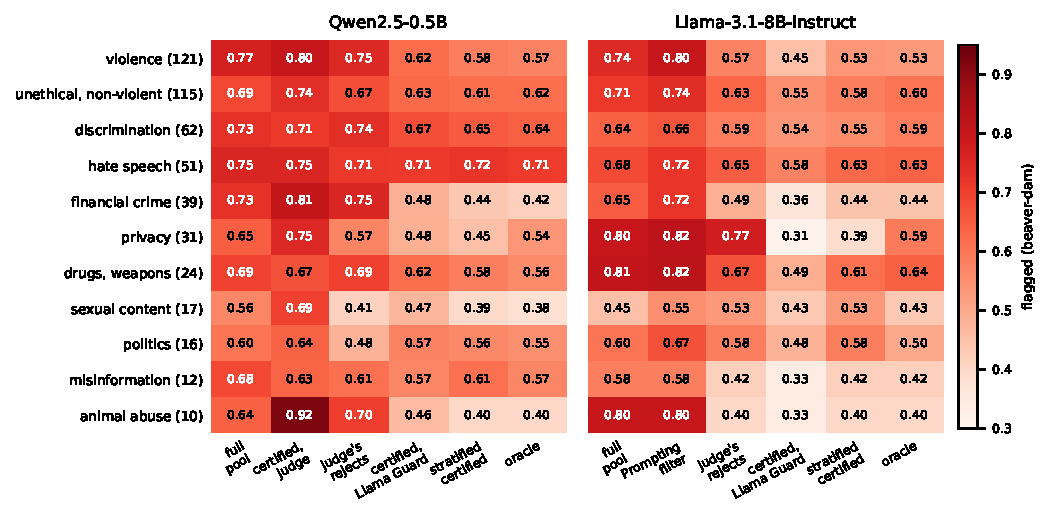
\includegraphics[width=\linewidth]{figures/categories.pdf}
\caption{Harm by prompt category for the six conditions of the diagnosis (every condition is in Tables~\ref{tab:step2} and~\ref{tab:field}): the fraction of held-out prompts flagged by beaver-dam among those whose human category label includes the category (number of prompts in parentheses; categories with fewer than $10$ prompts omitted), mean over seeds. The color scale spans the observed range; darker is more harmful.}
\label{fig:categories}
\end{figure}
Figure~\ref{fig:categories} splits the harm rate by the human category of the prompt, the convention of \citet{qi2024finetuning}. The $500$ held-out prompts carry BeaverTails' category mix (violence $121$, non-violent unethical behavior $115$, discrimination $62$, hate speech $51$, down to $10$ for animal abuse and fewer for child abuse, self-harm and terrorism, which are omitted), so the rates are conditional on the category and the small categories are noisy. In every category with at least $30$ prompts, at both scales, the judge-certified selection and the Prompting filter are within $0.02$ of or above the full pool, and the Llama Guard 3 certified and stratified conditions are within $0.07$ of or below the oracle. The reductions are largest for financial crime, violence and privacy ($0.3$ to $0.5$ from the full pool to the certified Llama Guard 3 condition at 8B) and smallest for hate speech and discrimination ($0.1$), which the oracle itself answers harmfully $0.63$ and $0.59$ of the time: what fine-tuning on curated data removes is the compliance the harmful examples teach, and the categories it moves most are the ones those examples concentrate in.

\section{Helpfulness and over-refusal}
\label{app:utility}
\begin{table}[h]
\centering\small
\caption{Helpfulness (ROUGE-L against human-safe reference responses) and XSTest refusal of safe prompts and harmful response to unsafe prompts for every condition of Table~\ref{tab:step2}, Qwen2.5-0.5B, mean $\pm$ standard error over its seeds.}
\label{tab:utility}
\tabinput{data/tables/utility.tex}
\end{table}
Table~\ref{tab:utility} reports ROUGE-L, the F1 of the longest common subsequence between the whitespace-tokenized, lowercased response and a reference, taken as the maximum over the human-safe reference responses of the prompt and averaged over the $229$ held-out prompts that have at least one; no judge model is involved.

\section{Stratified settings that refuse}
\label{app:strat}
Before the stratum-specific targets of Section~\ref{sec:strat}, we ran two settings fixed in advance: a two-property certificate on one walk (harmful fraction at most $0.10$ and safety-demonstration share at least $\beta$, Bonferroni $\delta/2$), which refuses everything at $n = 400$ with either scorer and at $n = 800$ for $\beta = 0.30$; and the stratified certificate at $\alpha = 0.10$ in both strata, which refuses at $n = 400$ and at $n = 800$ (Table~\ref{tab:strat}). Both refusals are correct: no Llama Guard 3 cutoff brings the harmful-prompt stratum below $10$ percent harmful on this pool. The targets $\alpha_h = 0.20$, $\alpha_b = 0.15$ were then fixed from the pool's stratum compositions before the calibration sample for the reported run was drawn, and the certificate's validity was re-verified on $200$ resampled draws at those targets (rate $0.70$, false certification $0.000$).

\section{A second pool}
\label{app:pool2}
\begin{table}[h]
\centering\small
\caption{The $0.5$B study on a pool of $4000$ from PKU-SafeRLHF at $\rho = 0.25$, three seeds. Bold and gray follow Section~\ref{sec:protocol}.}
\label{tab:pool2}
\resizebox{\linewidth}{!}{\tabinput{data/tables/pool2.tex}}
\end{table}
Table~\ref{tab:pool2} repeats the conditions of Tables~\ref{tab:step2} and~\ref{tab:strat} on a second pool: PKU-SafeRLHF \citep{ji2024pku} pairs, one Alpaca-7B response per prompt with its human safety label, $4000$ at $\rho = 0.25$, excluding the $152$ prompts shared with the $500$ evaluation prompts. The diagnosis of Section~\ref{sec:behavior} replicates: the judge-certified selection is certified on every seed at $6$ percent harmful and trains a more harmful model than the full pool under all four judges and on XSTest ($0.474$ against $0.439$ under beaver-dam), because it drops safety demonstrations ($0.29$ against $0.32$). The Llama Guard 3 selection, certified on every seed at $3$ percent harmful, keeps more demonstrations than the pool ($0.37$) and trains the safest curated model under the three judges that did not score it, within $0.01$ of the oracle ($0.384$ against $0.377$) with $400$ labels in place of $4000$. The stratified selection is certified on every seed and lands within $0.02$ of the pooled Llama Guard 3 condition, above it under those judges: on this pool the pooled scorer does not strip the demonstrations, so the stratified condition's extra demonstrations ($0.45$) do not pay for its extra harmful examples ($10$ percent against $3$), which is the trade-off Lemma~\ref{lem:tension} describes and the direction the aligned-model setting also shows.

\section{A second property}
\label{app:quality}
\begin{table}[h]
\centering\small
\caption{The certificate on response quality: Alpaca pools of $4000$, low quality as the property, certification rate against $n$ as measured/closed form over $200$ draws, $\delta = 0.1$, and the worst false-certification rate over the grid.}
\label{tab:quality}
\resizebox{\linewidth}{!}{\tabinput{data/tables/e7_quality.tex}}
\end{table}
The certificate takes any binary property with a scorer. Table~\ref{tab:quality} certifies response quality on Alpaca \citep{taori2023alpaca}: an example is low quality when it is absent from the AlpaGasus subset \citep{chen2023alpagasus}, in the public reimplementation whose GPT-4 rating kept $9{,}229$ examples, which makes $82$ percent of Alpaca low quality; the scorers are the same two Qwen judges asked whether the response is accurate, complete and helpful. Their AUROC on this property is $0.58$ to $0.61$, below their $0.72$ to $0.75$ on harmfulness. The certificate behaves as the theory says: the false-certification rate is at most $0.005$ in every setting; the natural pool and the $25$-percent pool at $\alpha = 0.10$ have negative margins and are refused at every budget; the $25$-percent pool at $\alpha = 0.25$ has margins of $0.08$ and $0.04$ and certifies at rates rising from $0.07$ to $0.87$ (7B judge) and $0.06$ to $0.43$ (1.5B judge) as $n$ goes from $50$ to $800$, with the closed form within $0.06$ of every measured rate (mean absolute error $0.005$ over $56$ settings). Predictions written before the run and their outcomes: validity (held), refusal on the natural pool (held), lower AUROC than on harmfulness (held), closed form within $0.02$ (held on average, not in every setting: the largest deviation is $0.06$). No model is fine-tuned on these selections: the result is that the certificate is property-agnostic, not a claim about quality-curated models.

\section{Instruction-style harm benchmarks}
\label{app:harmsets}
\begin{table}[h]
\centering\small
\caption{Every Qwen2.5-0.5B condition of Table~\ref{tab:step2} on DirectHarm4 ($400$ prompts), HarmBench's standard behaviors ($200$) and HEx-PHI's public release ($300$, ten of its eleven categories): beaver-dam flag rate per set and over all $900$, and the other three judges over all $900$; mean $\pm$ standard error over seeds. Bold and gray follow Section~\ref{sec:protocol}.}
\label{tab:harmsets05}
\resizebox{\linewidth}{!}{\tabinput{data/tables/harmsets_05b.tex}}
\end{table}
\begin{table}[h]
\centering\small
\caption{Every Llama-3.1-8B-Instruct condition of Table~\ref{tab:field} on the same three benchmarks, as in Table~\ref{tab:harmsets05}. Bold and gray follow Section~\ref{sec:protocol}.}
\label{tab:harmsets8}
\resizebox{\linewidth}{!}{\tabinput{data/tables/harmsets_8b.tex}}
\end{table}
\begin{figure}[h]
\centering
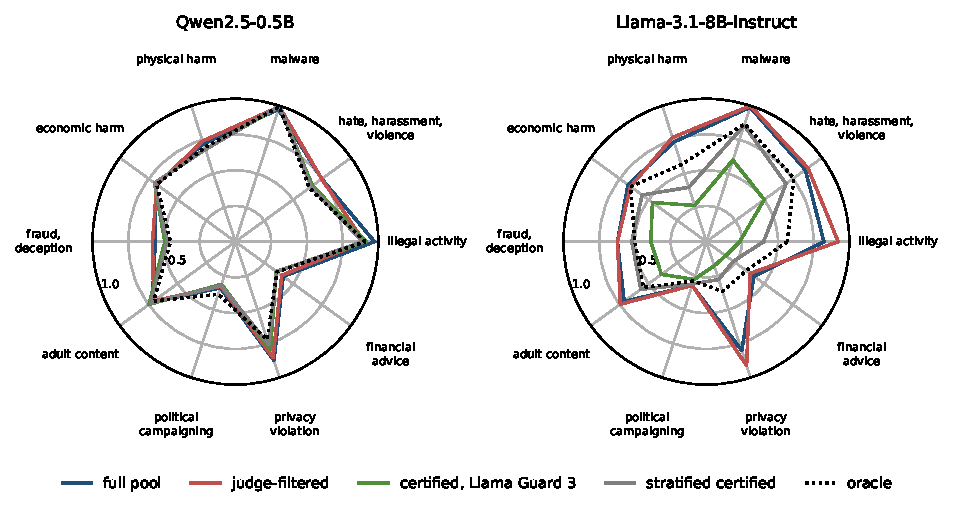
\includegraphics[width=\linewidth]{figures/hexphi.pdf}
\caption{Harm by HEx-PHI category ($30$ prompts each), beaver-dam flag rate, mean over seeds; judge-filtered is the judge-certified condition at 0.5B and the Prompting filter at 8B.}
\label{fig:hexphi}
\end{figure}
Tables~\ref{tab:harmsets05} and~\ref{tab:harmsets8} evaluate every condition on HEx-PHI \citep{qi2024finetuning}, HarmBench \citep{mazeika2024harmbench} and DirectHarm4 \citep{lyu2024directharm}, the harm benchmarks of \citet{zhang2026datashield} and \citet{larf2025}, generated and judged exactly as the BeaverTails prompts; Figure~\ref{fig:hexphi} splits HEx-PHI by its categories, which are balanced by construction. Predictions written before any generation and their outcomes: (1) the condition ordering on each set matches the BeaverTails ordering, Spearman at least $0.9$ under every judge: nearly held at 8B, where ten of the twelve (judge, set) pairs among the three judges that scored no condition clear the target and the other two are $0.886$ and $0.891$; failed at 0.5B ($0.053$ to $0.753$), where the fine-tuned conditions other than the oracle span only $0.04$; (2) the judge-filtered condition stays at or above the full pool on every set: held at 8B under every judge on the pooled benchmarks and on HEx-PHI, within $0.005$ below it on DirectHarm4 and HarmBench, failed at 0.5B ($0.643$ against $0.659$); (3) absolute rates higher than on BeaverTails, since every prompt is harmful: held; (4) the certified Llama Guard 3 and stratified conditions within $0.05$ of the oracle at 8B: the stratified condition is ($0.584$ against $0.626$), the certified condition is $0.16$ below it, failed in the safe direction. For the conditions added afterwards: SAFT's and SEAL's conditions are no safer than no filtering except through SAFT's degenerate seeds (held for SEAL; failed for SAFT, whose non-degenerate seeds, which keep $1004$ and $2519$ examples, land at $0.617$ and $0.678$ against $0.707$, consistent with the size effect of Section~\ref{sec:field}); every refused certified variant lands near random or no filtering and never below the Llama Guard 3 certified condition (held); the fixed Llama Guard 3 cutoff within $0.02$ of the certified condition at 8B (failed: $0.05$ apart on BeaverTails, $0.15$ on the benchmarks); labeled-only safer than the full pool and less safe than the oracle (failed: it is the safest condition in every column, Section~\ref{sec:field}).

\section{Contamination sweep under the aligned-model protocol}
\label{app:lambda}
\begin{table}[h]
\centering\small
\caption{Harm under beaver-dam in the aligned-model setting at three contamination levels, three seeds; certified seeds out of three in parentheses. Bold follows Section~\ref{sec:protocol}; SAFT's means include seeds that kept $24$ to $34$ examples and returned the untouched base model.}
\label{tab:lambda}
\tabinput{data/tables/lambda_sweep.tex}
\end{table}
\begin{figure}[h]
\centering
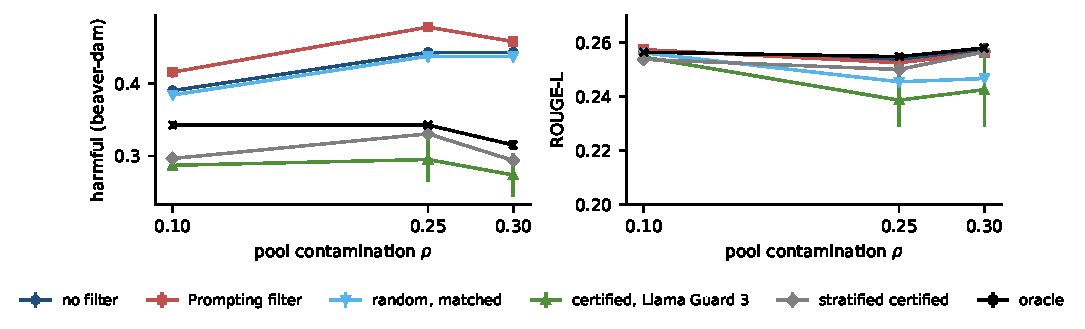
\includegraphics[width=\linewidth]{figures/lambda.pdf}
\caption{Aligned-model setting across pool contamination $\rho$: harm under beaver-dam (left) and ROUGE-L (right), mean $\pm$ standard error over three seeds.}
\label{fig:lambda}
\end{figure}
Table~\ref{tab:lambda} repeats the main $\rho = 0.25$ conditions at $\rho = 0.10$ and $0.30$: no filter, the Prompting filter, SAFT at both layers, random, the certificate on the SAFT score, and the pooled and stratified Llama Guard 3 certificates. SEAL, whose budget-matched selector costs nine GPU hours per pool, and the conditions added for completeness (the fixed Llama Guard 3 cutoff, labeled-only, the judge's rejects, the stratified certificate on the SAFT score, and the certified and stratified variants of the Prompting and SEAL scores) are run at $\rho = 0.25$ only. The Prompting filter is worse than no filtering at every level; the Llama Guard 3 certified conditions are the safest in the table at every level and below the oracle at every level; certification rates fall with contamination ($3/3$, $2/3$, $1/3$ for the pooled certificate), as the margin $\alpha - u_1$ shrinks. SAFT behaves at $\rho = 0.10$ and $0.30$ as at $0.25$: at $\rho = 0.10$ its cutoff removes almost nothing (it keeps $1669$ to $2773$ of $3000$ at $8$ to $9$ percent harmful, against the pool's $10$) and lands within $0.02$ of no filtering, and at $\rho = 0.30$ two of its three published-layer seeds keep $24$ and $25$ examples and return the base model, which is what its low mean in that column is. The certificate on SAFT's score refuses on every seed at every level; its fallback matches random at $\rho = 0.10$ and lands among SAFT's non-degenerate seeds at $0.30$ ($0.399$ against $0.39$ to $0.42$). Figure~\ref{fig:lambda} plots the conditions common to all three levels with ROUGE-L beside harm: at every level they span $0.13$ to $0.18$ in harm and at most $0.016$ in ROUGE-L, so the safety differences are not paid for in helpfulness.

\section{SAFT reimplementation and its Prompting baseline}
\label{app:saft}
\begin{figure}[h]
\centering
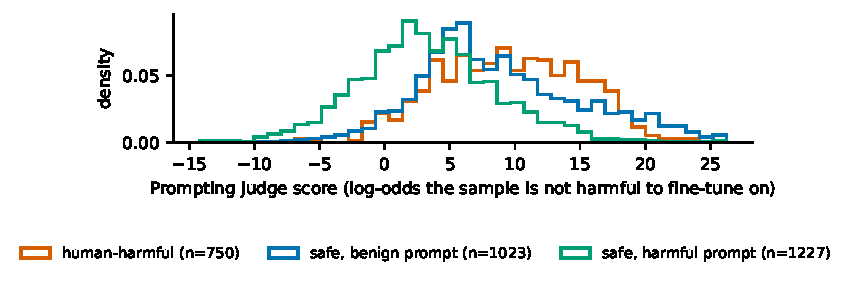
\includegraphics[width=0.75\linewidth]{figures/mechanism8.pdf}
\caption{The 8B analogue of Figure~\ref{fig:mechanism} (left): SAFT's Prompting judge on the $\rho = 0.25$ pool, by human label and prompt type.}
\label{fig:mechanism8}
\end{figure}
\paragraph{The Prompting judge.} Figure~\ref{fig:mechanism8} shows the score SAFT's Prompting baseline uses, the 7B judge asked whether a sample is harmful to fine-tune on, by group. The entanglement of Section~\ref{sec:behavior} is stronger here than at 0.5B: the judge scores human-harmful examples \emph{above} safe answers to harmful prompts on average, so a cutoff on its score removes safety demonstrations before harmful examples. In the terms of Lemma~\ref{lem:tension}, the judge retains demonstrations $0.58$ to $0.60$ times as often as harmful examples ($c < 1$) on the three certified-condition seeds, so no cutoff reaches $\alpha = 0.10$ (its certificate refuses, Table~\ref{tab:field}) and any selection that did would keep a demonstration share below $0.11$ against the pool's $0.55$ (\texttt{results/tension\_8b.json}).

No code accompanies \citet{choi2024saft}; we reimplemented it from the paper. Embeddings are the hidden state of the model to be fine-tuned at the start of the response section (their stated choice; the last token of the assistant header under Llama-3.1-8B-Instruct's chat template), from layer $15$ of $32$ (their best layer on Llama-2). The matrix of embeddings $e_i$ is centered and decomposed by SVD with right singular vectors $v_j$, the score is $s_i = d^{-1} \sum_{j \le d} \langle e_i, v_j \rangle^2$, and an example is removed when $s_i > \tau$; the subspace dimension $d \in \{1, 2, 3, 4\}$ and $\tau$ (one hundred candidates from the minimum to the maximum score) are chosen by F1 on $100$ labeled examples, as in their protocol. Where the paper is silent we fixed: the $100$ labeled examples are drawn from the pool and remain in the fine-tuning set (their labels set $\tau$ only), and F1 is the validation criterion. A second variant also validates the layer on the same labels, which on this model prefers the last layer on one seed. Table~\ref{tab:saftseeds} gives the per-seed outcome; the mean in Table~\ref{tab:field} is dominated by the degenerate seed. Figure~\ref{fig:saftkde} repeats SAFT's own diagnostic, the density of the score by label (their Appendix B), on our pool: at their layer the three groups overlap almost entirely, and at the last layer the score separates benign-prompt safe examples from harmful ones but places the safe answers to harmful prompts with the harmful examples, the same entanglement as the judge's. Predictions written before the run and their outcomes: AUROC near their published $0.69$ (outcome: $0.56$ to $0.61$); a large flagged fraction (outcome: $67$, $99$, and $16$ percent across seeds); harm between Prompting and the certified conditions (outcome: $0.40$ on the two non-degenerate seeds); refusal under the certificate on most seeds (outcome: all three). At 0.5B the same reimplementation on Qwen2.5-0.5B's embeddings (layer $12$ of $24$, $d$ and $\tau$ by F1 on $100$ labels) has AUROC at most $0.52$ over $d$ against the human label; its cutoff keeps $511$, $1104$, and $2345$ of $4000$ examples across seeds at $22$ percent harmful, and the models it trains are more harmful than the full pool under every judge ($0.475$ against $0.454$ under beaver-dam); under the certificate at $n = 400$ its score refuses on every seed and falls back to a set $26$ percent harmful that trains at the pool's level ($0.453$).
\begin{figure}[h]
\centering
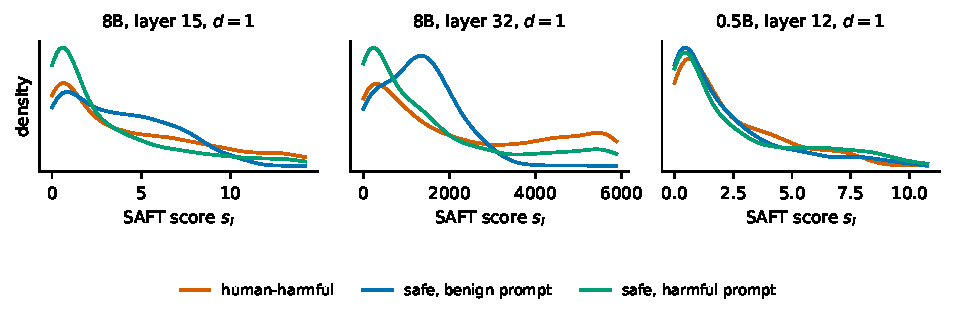
\includegraphics[width=0.85\linewidth]{figures/saft_kde.pdf}
\caption{Kernel density of SAFT's spectral score ($d = 1$) by human label and prompt type: the 8B pool at their layer (15 of 32) and at the last layer, and the 0.5B pool at layer 12 of 24.}
\label{fig:saftkde}
\end{figure}
\begin{table}[h]
\centering\small
\caption{SAFT per seed on the $\rho = 0.25$ pool.}
\label{tab:saftseeds}
\resizebox{\linewidth}{!}{\tabinput{data/tables/saft_seeds.tex}}
\end{table}

\section{SEAL}
\label{app:seal}
SEAL \citep{shen2025seal} learns one weight per example of the fine-tuning set by bilevel optimization: the lower level fine-tunes the model on the weighted set, the upper level evaluates it on a clean alignment set (BlueOrca in their release), and the weights move against the upper-level loss. We ran their public code with Llama-3.1-8B-Instruct (theirs: Llama-3-8B-Instruct), our $3000$-example pool as the set to be weighted, their BlueOrca release as the clean set, their LoRA rank, learning rates, batch size, and softmax selector, and their rule of keeping the top $80$ percent by selector weight, on one GPU: maximum length $512$ (theirs $1024$; only clean-set examples are truncated), ZeRO stage $0$ (single GPU), and torch AdamW in place of their fused Adam (no compiler on our machine; the same update). At their epoch count the selector's weights barely move, because an epoch in their loop is one pass over the set being weighted, $3000$ examples here against $112$k in their release, so the selector receives about $140$ updates instead of about $5000$. We therefore report two runs: their $3$ epochs, and $30$ epochs, which matches their number of selector updates on the smaller set. SEAL's AUROC against the human label is $0.52$ at $3$ epochs and $0.61$ at $30$; its top-$80$-percent selection is $24.4$ and $22.6$ percent harmful against the pool's $25$, and the models it trains are within $0.02$ of no filtering under every judge at both budgets (Table~\ref{tab:sealbudgets}; Table~\ref{tab:field} carries the $30$-epoch rows). The certificate on the $30$-epoch score refuses on all three seeds, as on the $3$-epoch score.
\begin{table}[h]
\centering\small
\caption{SEAL at both selector budgets, and its score under the pooled and stratified certificates, in the setting of Table~\ref{tab:field}. Bold: lowest harm per column among the SEAL conditions.}
\label{tab:sealbudgets}
\resizebox{\linewidth}{!}{\tabinput{data/tables/seal_budgets.tex}}
\end{table}

\section{Qualitative examples}
\label{app:qual}
Tables~\ref{tab:qual05} and~\ref{tab:qual8} show one held-out prompt per scale with the seed-0 response of fourteen conditions at 0.5B and seventeen at 8B, and the verdict of the two BeaverTails-trained judges ($\checkmark$ not flagged, $\times$ flagged). The prompt is chosen by a fixed rule rather than by hand: the first harmful held-out prompt, in evaluation order, whose no-filter response both judges flag and whose stratified certified response neither flags, with every response at most $320$ characters. At 0.5B the base model is weak and the conditions differ in degree; at 8B they differ in kind. A flag on a certified condition is not a failure of the certificate, which bounds the training set's composition and not the model's behavior: the judge-certified condition at 0.5B is the paper's central finding, and the SEAL-scored condition at 8B is a refusal that fell back to a selection its uninformative score could not improve.
\begin{table}[h]
\centering\scriptsize
\caption{Qwen2.5-0.5B, seed 0.}
\label{tab:qual05}
\tabinput{data/tables/qualitative_05b.tex}
\end{table}
\begin{table}[h]
\centering\scriptsize
\caption{Llama-3.1-8B-Instruct, $\rho = 0.25$, seed 0.}
\label{tab:qual8}
\tabinput{data/tables/qualitative_8b.tex}
\end{table}

\end{document}
